\section{Experiments}
The experiments compare the tests with various settings of match pairs in two aspects: \textit{effectiveness of property witnessing} and \textit{scalability of the algorithm}.
The match pairs in all the tests are generated by the new algorithm in this paper with different $k$. 
The encodings are solved by the SMT solver Z3 \cite{demoura:tacas08}. 

A series of experiments were conducted for seven typical benchmark programs that are either newly implemented or are employed by other papers \cite{benchmark:fevs,mpptest_benchmark,DBLP:conf/kbse/HuangMM13,DBLP:conf/ppopp/XueLWGCZZV09}. The benchmarks were tested for three types of properties: assertion violation, zero buffer compatibility and deadlock. 
%The results are shown in \tableref{table:benchmarks}. 
The initial execution trace for a CTP is generated by instrumenting the MPI programs with manually written scripts and executing the programs by MPICH \cite{mpich}, a public implementation of the MPI standard. The SMT encoding is generated by the rules in the prior work \cite{DBLP:conf/kbse/HuangMM13,HuangNFM15}. The deadlock testing requires a prior static analysis as preprocessing to find all the potential deadlock patterns in a program. 
The experimental results show a fair comparison among the deadlock tests for each benchmark as these tests are launched for the same deadlock pattern. 
%In precise, detecting assertion violation needs to encode the negation of user-provided assertions with respect of the computation in the program. Detecting zero buffer incompatibility needs to encode zero buffer semantics. The orphaned receive deadlock needs to encode the disjunction of the match pairs for each send for validating the potential deadlock. The assertion violation and the orphaned receive deadlock are tested under infinite buffer semantics. 
The experiments are run on a AMD A8 Quad Core processor with 6 GB of memory running Ubuntu 14.04 LTS. A time limit of 2 hours is set for each test. The test aborts the verification process if it does not complete within the time limit.

The results of the comparison are shown in \tableref{table:benchmarks} that divides the tests into three groups, where each group is the tests for a single type of property. Each group is labeled in the first column: ``AssertionV" means assertion violation; ``ZeroCom" means zero buffer compatibility; and ``DL" means deadlock. For each benchmark, the columns ``$k$", ``\#M", ``Time" and ``Speed" are measured for each of the three tests. The column ``\#M" is the number of the generated match pairs for $k$. The column ``Time" is for both constraint generation and solving. The notation ``TO" means ``time out" (exceeding the time limit set for each test). The column ``Speed" records the speedup that is computed by the simple formula in equation (4), where $\mathrm{Time}_\infty$ is the runtime of the SMT encoding with the over-approximated match pairs, and $\mathrm{Time}^\ast$ is computed in two ways. If the tested property does not exist in the benchmark, $\mathrm{Time}^\ast$ is the cumulative sum of a sequence, $\mathrm{Time}_1$, $\mathrm{Time}_2$, $\dots$, $\mathrm{Time}_k$, where each is the runtime of the encoding with a subscript representing the input for generating match pairs. If the property does exist, then $\mathrm{Time}^\ast$ is exactly $\mathrm{Time}_k$.
For the first case, it is possible that the value of Speed represents a slow down because the tests keep incrementing the value of $k$ and running the encodings with different inputs.
\begin{equation}
\mathrm{Speed} = \frac{\mathrm{Time_{\infty}}}{\mathrm{Time^{\ast}}}
\end{equation}
According to equation (4), a higher value of $\mathrm{Speed}$ indicates a shorter runtime of the encoding where the problem instance is simpler with the match pairs generated with $k$.
The symbol ``-" means that the $\mathrm{Speed}$ can not be computed because the test times out.

\begin{savenotes}
\begin{table*}[t]
\begin{center}
\scriptsize
\caption{Tests on Selected Benchmarks}\label{table:benchmarks}
     \begin{threeparttable}
     \def\arraystretch{1.5}
\begin{tabular}{c|c|c|c|p{0.25cm}|c|c|c|p{0.25cm}|c|c|c|c|c|c|c|}
		\cline{2-16}	  
& \multicolumn{3}{c|}{Test Programs} & \multicolumn{4}{c|}{Test 1} & \multicolumn{4}{c|}{Test 2} & \multicolumn{4}{c|}{Test 3}  \\ \cline{2-16}   
        & $Name$ & \#P & \#OP & $k$\tnote{w} & \#M & Time & Speed& $k$ & \#M & Time & Speed & $k$\tnote{+} & \#M & Time & Speed\\ \hline
         \multicolumn{1}{ |c|  }{\multirow{5}{*}{\rotatebox[origin=c]{90}{AssertV}}} 
          &  \textit{Diff2DNoBa} & 16 & 188 & 1\tnote{d} & 514 & 3.508s & 14.86 & 2\tnote{d}& 934 & 31.722s & 1.48 & 3\tnote{d}& 1,066 & 52.131s & 0.59 \\ \cline{2-16}
         \multicolumn{1}{ |c|  }{}&  \textit{DeepComm} & 5 & 180 & 1 & 240 & 0.837s & 1,647 & 5 & 960 & 10.547s & 131 & 15 & 2,760 & 1,379s & 1.00 \\ \cline{2-16}
\multicolumn{1}{ |c|  }{}&  \textit{Pktuse} &5 & 2048 &1 & 1,792 & 180s & $>$40 & 5   &    4,828      & 564s & $>$13 & 128 & 99,328 & TO & -- \\ \cline{2-16}
\multicolumn{1}{ |c|  }{}&  \textit{MultiM} & 3 & 266 & 1 & 500 & 10.892s & 295 & 5 & 1,300 & 24.397s & 132 & 100 & 20,300 & 3,218s & 1.00\\ \cline{2-16}
\multicolumn{1}{ |c|  }{}&  \textit{Floyd} &32 & 528 &1\tnote{d}& 1,928 & 29.925s & 0.97 & 2\tnote{d} &    1,928      & 30.621s & 0.48 & 3\tnote{d} & 1,928 & 29.043s & 0.32 \\ \hline
\hline
        
         \multicolumn{1}{ |c|  }{\multirow{7}{*}{\rotatebox[origin=c]{90}{ZeroCom}}} 
         &  \textit{Diff2DNoBa} & 16 & 188 & 1\tnote{d} & 514 & 1.749s & 3.07 & 2\tnote{d} & 934 & 3.053s & 1.12 & 3\tnote{d}& 1,066 & 5.375s & 0.53 \\ \cline{2-16}
        \multicolumn{1}{ |c|  }{} &  \textit{DeepComm} & 5 & 180 & 1 & 240 & 0.875s & 291 & 5 & 960 & 3.056s & 83 & 15 & 2,760 & 255s & 1.00 \\ \cline{2-16}
\multicolumn{1}{ |c|  }{}&  \textit{Pktuse} &5 & 2048 &1 & 1,792 & 121s & $>$59 & 5   &    4,828      & 449s & $>$16 & 128 & 99,328 & TO & -- \\ \cline{2-16}
\multicolumn{1}{ |c|  }{}&  \textit{MultiM} & 3 & 266 & 1 & 500 & 8.312s & 366 & 5 & 1,300 & 17.843s & 170 & 100 & 20,300 & 3,043s & 1.00\\ \cline{2-16}
\multicolumn{1}{ |c|  }{}&  \textit{Mismatch} &3 & 800 &1 & 204 & 2.904s & 3.06 & 30   &    622      & 3.297s & 2.69 & 50 & 793 & 8.872s & 1.00 \\ \cline{2-16}
\multicolumn{1}{ |c|  }{}&  \textit{MismatchEx} &3 & 296 &1 & 165 & 0.579s & 876  & 20   &    1,687      & 7.433s & 68 & 43 & 3,525 & 507s & 1.00  \\ \cline{2-16}
\multicolumn{1}{ |c|  }{}&  \textit{Floyd} &32 & 528 &1 & 1,928 & 89.032s & 1.02 & 5   &    1,928      & 90.908s & 1.00 & 10 & 1,928 & 91.155s & 1.00 \\ \hline
\hline

         \multicolumn{1}{ |c|  }{\multirow{3}{*}{\rotatebox[origin=c]{90}{DL}}} 
         &  \textit{Diff2DNoBa} & 16 & 188 & 1 & 514 & 3.479s & 13.50 & 2 & 934 & 44.060s & 1.07 & 3 & 1,066 & 46.974s & 1.00 \\ \cline{2-16}
\multicolumn{1}{ |c|  }{}&  \textit{Mismatch} &3 & 800 &1 & 204 & 2.160s & 6.61 & 30   &    622      & 10.061s & 1.42 & 50 & 793 & 14.286s & 1.00 \\ \cline{2-16}
\multicolumn{1}{ |c|  }{}&  \textit{MismatchEx} &3 & 296 &3 & 328 & 1.253s & 27.23 & 20   &    1,687      & 2.438s & 13.99 & 43 & 3,525 & 34.116s & 1.00 \\ \hline

       
\end{tabular}
\begin{tablenotes}
\item[w] $k$ is the minimum value with which the property is witnessed (if the property exists). 
\item[d] The property does not exist for the benchmark.
\item[+] The precise match pairs are over-approximated as $k$ is reached.
%\item[\textdagger] All the precise match pairs are required to witness a program zero buffer incompatible.
%\item[s] SMT analysis is not launched because no potential deadlock is detected in preprocessing.
%\item[a] No assertion is implemented in the program.
\end{tablenotes}
     \end{threeparttable}
\end{center}
\end{table*}
\end{savenotes}

Six typical benchmarks are tested. \textit{Diffu2DNoBa} is modified from the program \textit{Diffusion 2D}, which uses barriers to “partition” the message communication into several sections \cite{benchmark:fevs}. \textit{Diffu2DNoBa} removes the barriers from the original program. As such, deadlocks are present in the new program.

\textit{DeepComm} is a simple program with one receiver and 4 senders. In the program, the receiver issues 60 wildcard receives; each sender sends 15 messages to the receiver.
This scenario reflects the message non-determinism with 60 messages, such that the messages from different senders may race.

\textit{Pktuse} can be executed with 5 processes -- each of which randomly sends several messages to the other processes \cite{mpptest_benchmark}. The program uses wildcard receives only, therefore has a high degree of message non-determinism.

\textit{MultiM} is an extension to a program in the MCAPI library distribution \cite{DBLP:conf/kbse/HuangMM13}. The program adds extra iterations to the original program to generate longer execution trace. The assertions may be violated in possible executions.

\textit{Mismatch} implements the message communication that contains a deadlock. The program interleaves wildcard receives and deterministic receives in the program text. A deterministic receive may be orphaned in program execution leading to a deadlock as all the potential sends it need are matched with the preceding wildcard receives. 

\textit{MismatchEx} is an extension to the program in \figref{fig:example} that contains more sends and receives. The program also has a deadlock. 
%No assertions are present in the program.

\textit{Floyd} implements the shortest path algorithm for all the pairs of nodes \cite{DBLP:conf/ppopp/XueLWGCZZV09}. Each node communicates only with the immediate following neighbor. 

\subsection{Effectiveness}

The results show that each property, if existing for the benchmark, is efficiently witnessed by the SMT encoding with the under-approximated match pairs.  The tested properties for most programs can be witnessed with $k=1$. For example, the assertion violation for the program \textit{DeepComm} can be detected with $k=1$ where the speedup (1,647) is very high. 
The algorithm, although is unable to detect the deadlock for the program \textit{MismatchEx} with $k=1$, has a quick response when this deadlock is witnessed with $k=3$.

%Another example is the deadlock test for the program \textit{Mismatch}. 
%The deadlock can be detected around 2 seconds for $k=1$, while the encoding with $k=50$ needs to run 14 seconds for the same property. 

For the tests where the properties do not exist in the benchmarks, the results show a certain degree of slow down. For example, the assertion violation test for the program \textit{Diffu2DNoBa} takes about 3 seconds to complete for $k=1$. Since no property is witnessed at the initial iteration, the algorithm raises $k$ to $2$, and repeats the match set generation and the encoding solving until the match pairs are over-approximated, which in this case, is that $k$ is equal to $3$. As the runtime is cumulated from $k=1$ through $k=3$, the speedup is less than $1$, indicating a slow down from the runtime of the encoding with the over-approximated match pairs.
 
%also show that the runtime cost of the encoding is highly reduced with the match pairs generated with smaller $k$. For example, the assertion violation test for the program \textit{Diffu2DNoBa} takes 3 seconds to complete for $k=1$, while it takes to 67 seconds to solve the same encoding for $k=5$ only the match set is larger.

%To check zero buffer incompatibility, the precise match pairs are required because a zero buffer incompatible program indicates that all possible schedules are infeasible under zero buffer semantics. 
%As such, the zero buffer incompatibility for the program \textit{Diff2DNoBa} is only detected with $k=\infty$. 
%On the other hand, if any schedule for a program is able to run under zero buffer semantics, the program may never be zero buffer incompatible. As such, if a test shows that a zero buffer encoding is satisfiable for the program, then the program is proved to be zero buffer compatible. 
%The results show that the benchmarks excluding the program \textit{Diff2DNoBa} are zero buffer compatible by testing them with only a small set of match pairs.

%For deadlock detection, a prior static analysis is launched as preprocessing to find all the potential deadlocks in a program. If no potential deadlocks are found, then the SMT encoding is not required. For example, the deadlock test for the program \textit{MuitiM} is unavailable because no potential deadlock is detected.

\begin{figure}[!h]

\begin{minipage}{.55\textwidth}
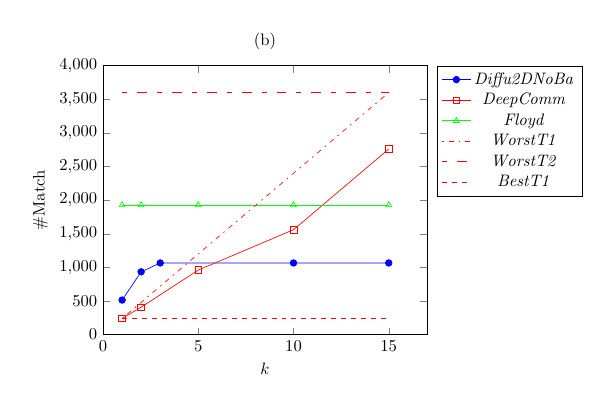
\begin{tikzpicture}[scale=0.6]
\begin{axis}[
   title = {(b)},
    xlabel={$k$},
    ylabel={\#Match},
    xmin=0, xmax=17,
    ymin=0, ymax=4000,
    xtick={0,5,10,15},
    xticklabels={0,5,10,15,20,25,30,35,40,$\infty$},
    ytick={0,500,1000,1500,2000,2500,3000,3500,4000},
    legend pos= outer north east,
    %ymajorgrids=true,
    grid style=dashed,
]
 
\addplot[
    color=blue,
    mark=*,
    ]
    coordinates {
    (1,514)(2,934)(3,1066)(10,1066)(15,1066)
    };
    
\addplot[
    color=red,
    mark=square,
    ]
    coordinates {
    (1,240)(2,408)(5,960)(10,1560)(15,2760)
    };
    
   
    
\addplot[
    color=green,
    mark=triangle,
    ]
    coordinates {
    (1,1928)(2,1928)(5,1928)(10,1928)(15,1928)
    };
    
     \addplot[
    color=red,
                dash pattern=on 1pt off 3pt on 3pt off 3pt,
    ]
    coordinates {
    (1,240)(2,480)(5,1200)(10,2400)(15,3600)
    };
    
     \addplot[
    color=red,
                dash pattern=on 3pt off 6pt on 6pt off 6pt,
    ]
    coordinates {
    (1,3600)(2,3600)(5,3600)(10,3600)(15,3600)
    };
    
     \addplot[
    color=red,
    dashed,
    ]
    coordinates {
    (1,240)(2,240)(5,240)(10,240)(15,240)
    };
    
    \legend{\textit{Diffu2DNoBa},\textit{DeepComm},\textit{Floyd},\textit{WorstT1},\textit{WorstT2},\textit{BestT1}}
\end{axis}
\end{tikzpicture}
\end{minipage}
\begin{minipage}{.5\textwidth}
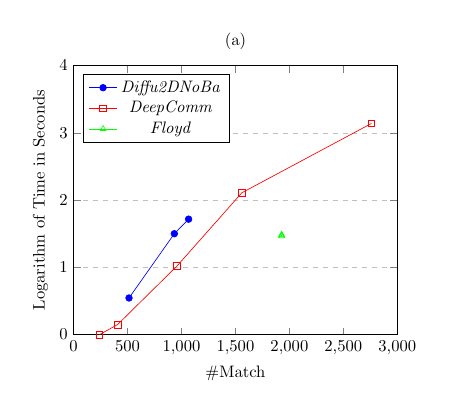
\begin{tikzpicture}[scale=0.6]
\begin{axis}[
title = {(a)},
    xlabel={\#Match},
    ylabel={Logarithm of Time in Seconds},
    xmin=0, xmax=3000,
    ymin=0, ymax=4,
    xtick={0,500,1000,1500,2000,2500,3000},
    ytick={0,1,2,3,4},
    legend pos= north west,
    ymajorgrids=true,
    grid style=dashed,
]
 
\addplot[
    color=blue,
    mark=*,
    ]
    coordinates {
    (514,0.545)(934,1.501)(1066,1.717)
    };

\addplot[
    color=red,
    mark=square,
    ]
    coordinates {
    (240,0)(408,0.149)(960,1.023)(1560,2.110)(2760,3.140)
    };

\addplot[
    color=green,
    mark=triangle,
    ]
    coordinates {
    (1928,1.476)(1928,1.486)(1928,1.463)
    };
    \legend{\textit{Diffu2DNoBa},\textit{DeepComm},\textit{Floyd}}
 
\end{axis}
 
\end{tikzpicture}
\end{minipage}
\caption{(a) The number of match pairs of varying the input $k$. (b) The logarithm of the time for assertion violation detection of varying the number of match pairs.}
\label{fig:relation}
\end{figure}

\subsection{Scalability}

To evaluate how the input $k$ impacts the number of the generated match pairs and the runtime cost of SMT encoding, the plots in \figref{fig:relation} show the relations for three benchmarks. 
These relations are plotted from both the experimental data in \tableref{table:benchmarks} and additional test data if needed. \figref{fig:relation} (a) shows the relation between the input $k$ and the number of the generated match pairs. 

To better explain the plots in \figref{fig:relation} (a), the presentation discusses two types of worst case for message passing programs. 
The first type is related to message non-determinism. 
It is assumed that a program has $\mathit{NR}_t$ receives and $|frm_t|$ senders for each process $p_t$. Also assuming that $|frm_t|\times k < \mathit{NR}_t$ for a set of possible values of $k$. As such, there are $|frm_t|\times k$ receives in each section, and therefore $\frac{\mathit{NR}_t}{|frm_t|\times k}$ sections for $p_t$.
If all the receives are wildcard, which is the worst case of message non-determinism, then the size of the generated match set for each section is $O(|frm_t|^2\times k^2)$ as the complexity of $\mathrm{MatchApprox}$ in \algoref{algo:main} is quadratic. 
As such, the size of the match set for all the sends and receives in $p_t$ is $O(\frac{\mathit{NR}_t}{|frm_t|\times k} \times |frm_t|^2\times k^2) = O(\mathit{NR}_t \times |frm_t| \times k) = O(k)$ as $\mathit{NR}_t$ and $|frm_t|$ are constants. 

\textit{WorstT1} in \figref{fig:relation} (a) shows an example of the worst case of message non-determinism, where the program issues 60 receives among 5 processes, and each process has four senders. 
As shown, the number of the generated match pairs for \textit{WorstT1} grows linearly as $k$ increases. 
The growth of \textit{DeepComm} in \figref{fig:relation} is close to \textit{WorstT1}, where they have the same number of messages, the same number of processes, and the same number of senders for each process.

In contrast, the best case of message non-determinism is a program that contains only the deterministic receives. 
As such, the size of the match set for each section is equal to the number of receives in each section ($|frm_t|\times k$). Therefore, the number of the generated match pairs for $p_t$ is $\mathit{NR}_t$ for any possible $k$. \textit{BestT1} shows  the best case for the program with the same program configuration of \textit{WorstT1} except that all the receives are deterministic.
No benchmark in \figref{fig:relation} is close to the best case as the programs with few or no degree of message non-determinism is not interesting for testing.  

The second type of worst case is related to deep communication between any two processes. Deep communication in this context means a process may receive many messages from each single sender.
One of the assumptions in the first type of worst case is that $|frm_t|\times k < \mathit{NR}_t$, indicating that each sender is able to send more than $k$ messages to the receiver $p_t$. 
If only wide communication is implemented for $p_t$ meaning that each sender can only send one message to $p_t$, which is the worst case of deep communication, then the number of the distributed sends for each section is $\mathit{NR}_t$ according to equation (3). 
As a result, there is only one ($\frac{\mathit{NR}_t}{\mathit{NR}_t} = 1$) section for each process $p_t$. 
In this situation, the number of the generated match pairs for $p_t$ is $|M|$ for any possible $k$, where $M$ is the match set for $p_t$ by applying the over-approximation function $\mathrm{MatchApprox}$ in \algoref{algo:main}. 
\textit{WorstT2} in \figref{fig:relation} (a) shows an example of the worst case of deep communication, where the program has 60 wildcard receives in the first process, and each of the other 60 processes only sends a single message to the first process. 
The program \textit{Floyd} in \figref{fig:relation} (a) is also in this type of worst case. 

As for the best case of deep communication, the program has to contain only the deep communication but not the wide communication. There is no message non-determinism in such a program because only one sender exists for each receiver so the messages are received in a fixed FIFO order.

The program \textit{Diff2DNoBa} shows a certain degree of both cases in \figref{fig:relation} (a). For message non-determinism, the the program has a sharp growth between $k=1$ and $k=2$, and then grows more gently until $k=3$. The growth is not linear because both wildcard receives and deterministic receives are implemented in the program. For deep communication, the number of match pairs for this program reaches the limit when $k=3$. The limit represents the largest set of match pairs that can be generated by the algorithm. The algorithm rapidly reaches the limit for this program because more wide communication are employed than the deep communication.  

\figref{fig:relation} (b) illustrates the relation between the number of the generated match pairs and the logarithm of the runtime for assertion violation tests. 
For the programs \textit{Diffu2DNoBa} and \textit{DeepComm}, the plots both show linear growth, indicating that the runtime increases exponentially as the number of match pairs grows. 
This observation demonstrates that the test is scalable only if the number of match pairs is small. 
Note that the plots for the program \textit{Floyd} are overlapped because the number of the generated match pairs is identical for each test.
According to the two diagrams in \figref{fig:relation}, the algorithm is able to scale to the program with a high degree of message non-determinism and a high degree of deep communication if the input $k$ is small.
